
%%%%%%%%%%%%%%%%%%%%%%%%%%%%%%%%%%%%%%%%%%%%%%%%%%%%%%%%%%%%%%%%%%%%%%%%%
%           Capítulo 2: MARCO TEÓRICO - REVISIÓN DE LITERATURA
%%%%%%%%%%%%%%%%%%%%%%%%%%%%%%%%%%%%%%%%%%%%%%%%%%%%%%%%%%%%%%%%%%%%%%%%%

\chapter{Marco teórico}
\section{La Gestión de Inventarios}

La empresa tiene la necesidad de saber en cantidad monetaria cuanto es lo que tiene en ingresos y cuanto es lo que tiene en gastos. Por eso es importante que la empresa pueda tener registros de cada una de sus actividades, ya sea de actividades que generan ingresos como las que generan egresos. En este sentido, llega a ser necesario que se tenga un registro de esas actividades, aunque ello conlleve costos adicionales. \citep{FundGeInv}\\

La gestión de inventarios es un proceso que una empresa puede asumir o no. Se dice que mantener un inventario tiene un costo asociado y también se tiene un costo por no mantener una gestión de inventarios. \citep{FundGeInv}\\

Se hace una diferencia entre inventarios para empresas de producción y también para empresas comerciales. En empresas de producción o industriales, el costo de inventarios puede representar el 40\% de su capital invertido. En una empresa comercial este costo puede alcanzar el 70\% de su capital invertido representado en su mercancía o mercadería. \citep{FundGeInv}\\

La gestión de almacenes cumple con las funciones de ser un procesos que sincroniza la oferta y la demanda, también tiene la función de reducir costes, mediante la compra de grandes lotes que hacerlo por pequeños lotes. En ocasiones también tiene la función de ser parte del proceso de la empresa en la producción de algún bien. \citep{FundGeInv}

\section{Clasificación de Inventarios}

Es posible clasificar los almacenes según varios criterios y por lo tanto es posible tener varios tipos de almacenes.  Almacenes principales o centrales,  Almacenes subsidiarios o periféricos. Depósitos y almacenes móviles.

\section{Organización de Inventarios}

La organización de inventarios tiene dos puntos de vista que son de acuerdo a la organización administrativa y al flujo de los materiales.\\

Desde la segunda consideración señalada, la organización de los almacenes debe tener en cuenta las siguientes consideraciones: [\citep{UDL:2019:Online}]

\begin{enumerate}
\item Ya que el almacén, tal como ya se ha dicho, no es un ente aislado, su planificación deberá ser acorde con las políticas y objetivos generales de la empresa.
\item Se deben vigilar las cantidades almacenadas, equilibrando costes y servicio.
\item Su disposición permitirá minimizar los esfuerzos para su funcionamiento, para ello deberán tenerse en cuenta elementos tales como el espacio empleado, el tráfico interior, los movimientos a efectuar y los riesgos o condiciones ambientales y de seguridad.
\item Su estructura e implantación deberá ser lo suficientemente flexible como para permitir nuevas adaptaciones a las necesidades que la evolución del tiempo determine.
\end{enumerate}

Como norma general, todo almacén deberá satisfacer los siguientes requisitos mínimos:

\begin{itemize}
\item Una recepción cómoda de los materiales.
\item Unas instalaciones adaptadas al tipo de material almacenado y a sus exigencias de manipulación.
\item Posibilidad de una fácil distribución.
\end{itemize}

Por otra parte, se debe tener en cuenta que un almacenamiento inadecuado puede presentar los siguientes problemas:

\begin{itemize}
\item Confusiones, tanto en la sistematización de las mercancías como en la identificación de las mismas.
\item Congestión del tráfico de materiales.
\item Peligro de sobrecarga de las diferentes plantas que puede tener.
\item Mayor riesgo de incendio o de deterioro.
\item Problemas de conservación del material depositado de forma inadecuada.
\item Dificultad para la rotación de los materiales.
\item Despilfarro de movimientos y desplazamientos.
\item Mala utilización de los medios y del personal, etc.
\end{itemize}

Los métodos de valoración de inventarios son técnicas utilizadas con el objetivo de seleccionar y aplicar una base específica para valuar los inventarios en términos monetarios. La valuación de inventarios es un proceso vital cuando los precios unitarios de adquisición han sido diferentes.\\

Existen numerosas técnicas de valoración de inventarios, sin embargo las comúnmente utilizadas por las organizaciones en la actualidad (dada su utilidad) son:

\begin{itemize}
\item Identificación Específica 
\item Primeros en Entrar Primeros en Salir - PEPS
\item Últimos en Entrar Primeros en Salir - UEPS
\item Costo promedio constante o Promedio Ponderado.
\end{itemize}

\section{Pasos para realizar un inventario}

\begin{enumerate}
\item Identificar los bienes a inventariar: El primer paso es tener claro que bienes son los que corresponde inventariar y que bienes no.
\item Determinar los lugares a inventariar: Una vez aclarado cuáles son los bienes que corresponde incluir en el inventario, habrá que tener presente todos los lugares en los que están para no omitirlos. Otra recomendación de índoles metodológica, teniendo en cuenta la cantidad de lugares por los que deberemos pasar al hacer inventario: nos conviene con anticipación recorrer esos lugares y ordenarlos, si es que no lo están, a fin de poder identificar sin problemas los bienes y evitar reiteraciones u omisiones.
\item Armar un equipo de trabajo: Consideramos de suma importancia este tema porque además de hacer la tarea de manera más eficiente, es una muestra de solidaridad y corresponsabilidad por parte de las personas que hacen parte del almacén.
\item Recorrido, recuento y registro: Una vez cumplidos los pasos anteriores estamos en condiciones de comenzar el inventario propiamente dicho. Para ello se fijará un día y hora en que se llevará a cabo (es importante cuidar el detalle de que sea en el mismo momento en toda la comunidad). Es importante que se familiaricen con las planillas a utilizar, dado que estas deben convertirse en una ayuda que facilite el trabajo, no en un obstáculo. Un detalle a tener en cuenta es el riesgo de no inventariar algún objeto, o de contarlo más de una vez. Para que esto no suceda, lo ideal es dejar algún tipo de marca que indique con claridad que ese ítem ya fue contado.
\end{enumerate}

Cada equipo de trabajo definirá cual es la mejor manera de hacerlo, la que más se adecue al tipo de bien de que se trate, tal vez colocar una etiqueta o una cinta o tarjeta remisible podrían ser algunos caminos a seguir.

\section{El producto}

La empresa dependiendo a la función que se dedica o al tipo de empresa, expresa de manera diferente el concepto de producto. Para una empresa que fabricación, el producto es lo que “fabrica” y es para cubrir una necesidad de sus clientes. En cambio en una empresa que comercializa el concepto puede ser un bien que cubre una necesidad que sus clientes requieran. [\citep{UDL:2019:Online}]\\

Sin embargo el concepto de producto puede ser muy amplio, como se define en [\citep{UDL:2019:Online}] que indica\\

\begin{center}
    \begin{minipage}{0.9\linewidth}
        \vspace{5pt}
        {\small
            Cualquier bien material, servicio o idea que posea un valor para el consumidor y sea susceptible de satisfacer una necesidad.
        }
        \begin{flushright}
            (\citeauthor{PrinStraMark}: 211)
        \end{flushright}
        \vspace{5pt}
    \end{minipage}
\end{center}

Esta definición llega a ser demasiado extensa al propósito de modelar un sistema de gestión de almacenes, sin embargo podemos obtener características que pueden ayudar a definir un sistema de gestión.

\subsection{Precio y costo del producto}

La finalidad de la empresa está en generar beneficios a los participantes. Bajo este sentido se tiene definido el precio y costo de un producto y la diferencia entre estos valores se puede obtener una ganancia. La ganancia puede considerarse como un beneficio, teniendo en cuenta que puede haber más beneficios, tanto para la empresa como para los clientes de estos mismos.\\

El precio es el valor monetario para que los clientes puedan adquirir el producto. El costo es visto desde el punto de vista de la empresa como el valor que tuvo que pagar la empresa para fabricar o para conseguir el producto. Esta última definición es sí, se trata de una empresa de comercialización.\\

Tanto el valor del precio de un producto como su costo están incluidos en teorías y procedimientos para obtenerlos, también pueden basarse en el mercado en el cual son comercializados e incluso de otros factores que no analizaremos en este documento ya que se salen del propósito del mismo [\citep{PrinStraMark}]\\

En un marco de almacenamiento, se necesita conocer el precio y el costo, ya que el propósito esencial de la gestión de materiales es saber cuánto se tiene almacenado en términos monetarios; cuanto se tiene en proceso si de una empresa de fabricación se trata. Estos valores son manejados metódicamente para permitirnos un cálculo en función a su movimiento, a su costo, a su localización, al volumen que ocupa, al material del que está compuesto e incluso otros factores más que salen del propósito de esta tesis.\\

Para aclarar un poco todo lo expuesto anteriormente, los elementos que pueden influir en el costo de almacenar están los siguientes
El paquete que puede contener al producto, que incluye su volumen, medidas del paquete, su peso y su material; que puede ser líquido o sólido.\\

Su posición física, que puede ser dentro de la empresa o el algún almacén, la distancia, para recorrer, el tiempo para preparar su transporte.\\

En fin, todo lo anterior se puede resumir en una palabra y es la logística. [\citet{LogAdmiCadSumi}]

\subsection{Código de barras}

En el proceso de almacenes, es útil tener un registro de cada uno de los elementos que interesen en el mismo. Este registro se hace individualmente a cada producto que se almacena. Para efectuar dicho registro es útil hacer uso de los códigos de barras. Los códigos de barras son imágenes que de manera estándar identifican un producto de manera única en todo el mundo.
Se tienen varios estándares para los códigos de barras, el más común es EAN/UPC (EAN International – Uniform Code Council). [\citep{BPS:2019:Online}]\\

Entre las ventajas del uso de código de barras en almacenes esta que este proceso es más preciso con información valiosa, reduciendo el tiempo que toma un proceso de inventariado.

\subsection{Uso del código de barras}

El empleo de códigos de barras puede ser diversos, no solamente de la cantidad logística. Permite tener un control de las localizaciones de cada producto, de unidades de comercialización e incluso de los activos de una empresa.\\ [\citep{CCCB:2019:Online}]

En la siguientes secciones trataremos de mostrar una explicación más profunda del uso de los códigos de barras.\\

\subsection{Catálogos de productos}
En la creación de catalogos de productos el uso de código de barras pude ser empleado de la siguiente manera. \citep{CCCB:2019:Online}

\begin{enumerate}

\item Creación de una referencia interna. No importa su longitud, ni si es alfanumérica. Cuanto más esclarecedora sea para su empresa, mejor. A la hora de crear un catálogo se deben tener en cuenta todos los niveles de agrupación en los que estos productos sean susceptibles de ser comercializados. (Ilustración: ejemplo de un catálogo con 3 columnas: referencia interna, descripción y GTIN)

\item Añadir una segunda columna con la descripción del producto. Ésto facilitará a sus interlocutores el conocimiento de sus artículos.

\item Una vez realizado el ejercicio anterior, el siguiente paso es proceder a la codificación de todos los artículos contenidos en el catálogo de la empresa mediante la asignación de un GTIN.
\end{enumerate}

\begin{figure}
  \centering
    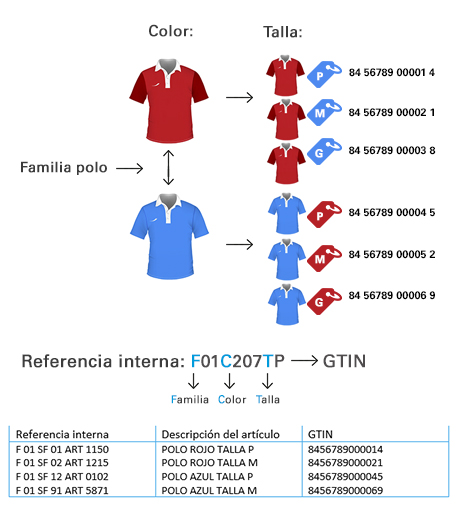
\includegraphics[scale=0.5]{./Capitulo2/figs/catalogo_post_barras.jpg}
  \caption{Referencia interna para la estructura de código de barras en la creación de catálogs de productos.}
  \label{catalogo_post_barras}
\end{figure}

\subsection{Codificaciones de agrupaciones}

Una agrupación es un conjunto de unidades de consumo cuya función es facilitar el manipulado de éstas, tanto en lo que se refiere a los envíos, como a los procesos de entrega, recepción, etc.\\

Todas las agrupaciones pueden ser separadas en las unidades de consumo que las forman.\\

Es correcto identificar una agrupación asignando un código GTIN-13 que identifique a la misma, distinto al de la unidad de consumo que contiene.\\

También es posible identificar la agrupación mediante un código GTIN-14. Éste se obtiene añadiendo delante del GTIN-13 de la unidad de consumo una Variable Logística.\

La variable logística es el dígito situado a la izquierda del código GTIN-14 de la unidad de consumo.\\

Los valores que puede tomar están entre el 1 y el 8, ambos inclusive.\\ [\citep{CCCB:2019:Online}]

\begin{figure}
  \centering
    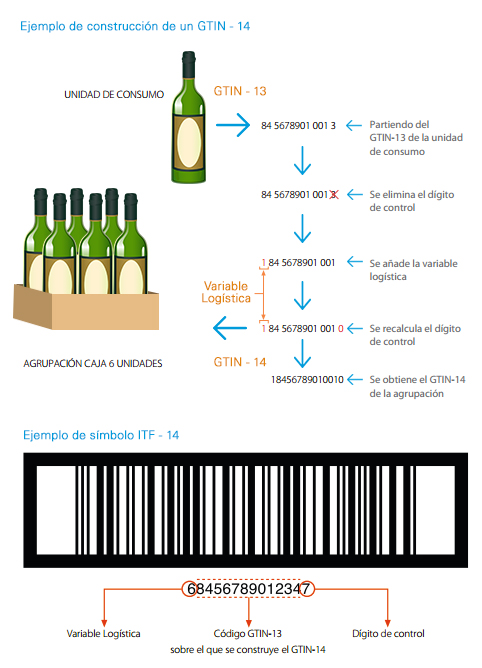
\includegraphics[scale=0.5]{./Capitulo2/figs/codificacion_agrupaciones_post_barras.jpg}
  \caption{La codificación de agrupaciones permite manipular un conjunto de unidades, que puede ser útil para su manipuleo y transporte.}
  \label{codificacion_agrupaciones_post_barras}
\end{figure}
